\apendice{Resultados estudio}

\section{Introducción}

En este apartado se detallaran las pruebas realizadas durante el desarrollo de la aplicación para mostrar su funcion.

\section{Comparativa de algoritmos}

Tras la optimización del algoritmo pero antes de la implementación a la pagina web, se buscó comparar el funcionamiento y los resultados que podían proporcionar los diferentes algoritmos de clustering bajo condiciones relativamente equivalentes. Para ello, se utilizó la misma cantidad de datos: doscientas filas del archivo \texttt{Trayectorias Taxis} \cite{trayectorias_taxis}. Respecto a los parámetros necesarios para la ejecución de cada algoritmo, se intentó mantenerlos lo más estándar posible. Por ejemplo, en los casos en que era necesario especificar el número de clusters, se utilizó una aproximación basada en el resultado obtenido por OPTICS, ya que este algoritmo no requiere definir dicho parámetro. El resto de los parámetros se dejaron en los valores predeterminados que proporciona la biblioteca \texttt{scikit-learn}.

Aunque se probaron más algoritmos, solo cinco llegaron a la etapa final del desarrollo de la página web. Algunos, como \textbf{Birch}, no lograron producir resultados satisfactorios, aunque se considera que, con una adaptación más específica de los datos, podrían haber funcionado correctamente.

A continuación, se describen los resultados obtenidos para cada uno de los algoritmos seleccionados:

\begin{enumerate}

\item \textbf{OPTICS}:  
Este fue el primer algoritmo probado de manera intensiva, ya que era el utilizado por defecto en la implementación base. De las doscientas filas procesadas, se generaron un total de 2161 segmentos, que fueron agrupados en 106 clusters. Sin embargo, no todos los segmentos se utilizaron para la creación de los clusters; un total de 1354 segmentos fueron catalogados como "basura", lo que corresponde al 62.66\% de los datos. A continuación, se muestran los resultados en tres imágenes diferentes: la representación de los clusters, un histograma con la cantidad de trayectorias que forman cada cluster y la representación de trayectorias generadas por el algoritmo TRACLUS.

\begin{figure}[h!]
    \centering
    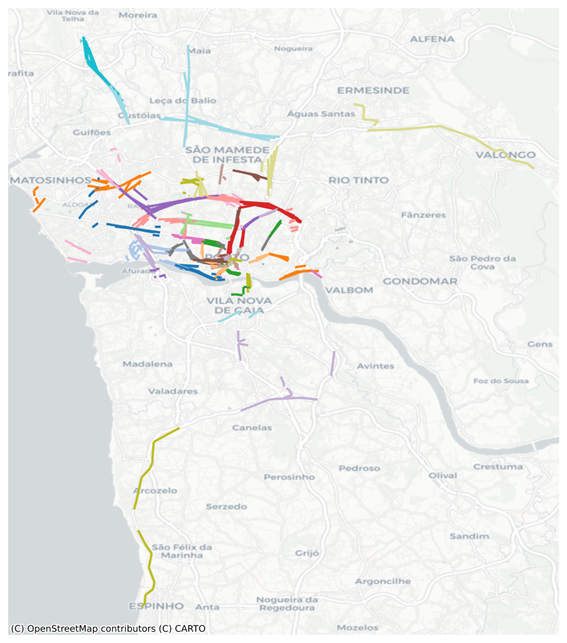
\includegraphics[width=0.5\textwidth]{img/clusters_OPTICS.png}
    \caption{Representación de clusters.}
    \label{fig:clusters_OPTICS}
\end{figure}

\begin{figure}[h!]
    \centering
    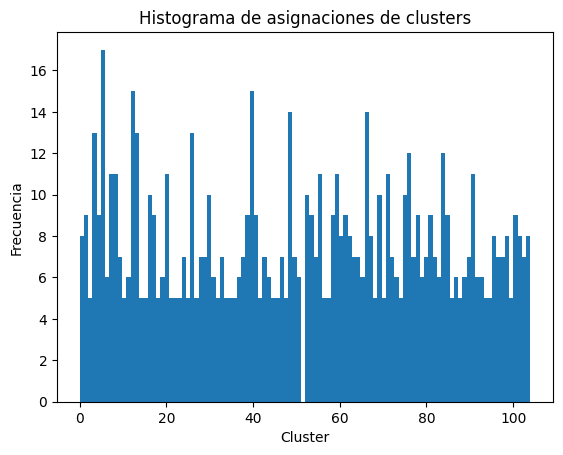
\includegraphics[width=0.5\textwidth]{img/histograma_OPTICS.png}
    \caption{Segmentos por cada cluster.}
    \label{fig:histograma_OPTICS}
\end{figure}

\begin{figure}[h!]
    \centering
    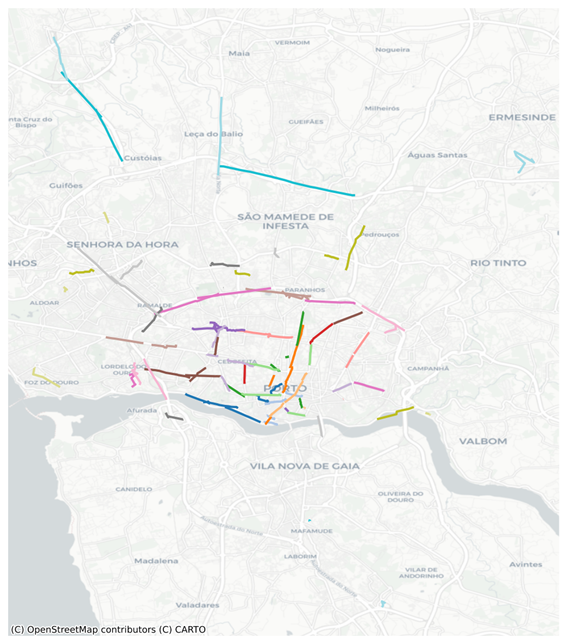
\includegraphics[width=0.5\textwidth]{img/r_tray_OPTICS.png}
    \caption{Representación de trayectorias.}
    \label{fig:trayectorias_OPTICS}
\end{figure}

\FloatBarrier

\item \textbf{DBSCAN}:  
Con un valor de \texttt{eps} de 0.1, los resultados de DBSCAN fueron significativamente diferentes a los de OPTICS. Aunque se generaron más segmentos (2654 en total), el número de clusters disminuyó a 37. Además, el porcentaje de datos clasificados como "basura" aumentó al 90.09\%, lo que equivale a 2391 segmentos descartados.

\begin{figure}[h!]
    \centering
    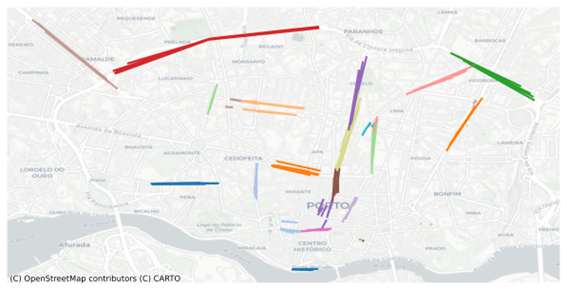
\includegraphics[width=0.5\textwidth]{img/clusters_DBSCAN.png}
    \caption{Representación de clusters.}
    \label{fig:clusters_DBSCAN}
\end{figure}

\begin{figure}[h!]
    \centering
    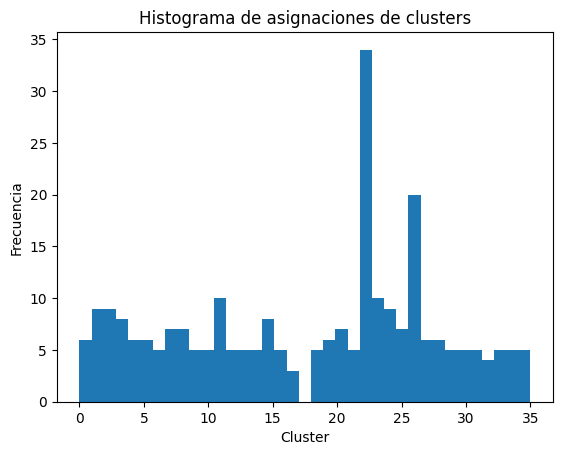
\includegraphics[width=0.5\textwidth]{img/histograma_DBSCAN.png}
    \caption{Segmentos por cada cluster.}
    \label{fig:histograma_DBSCAN}
\end{figure}

\begin{figure}[h!]
    \centering
    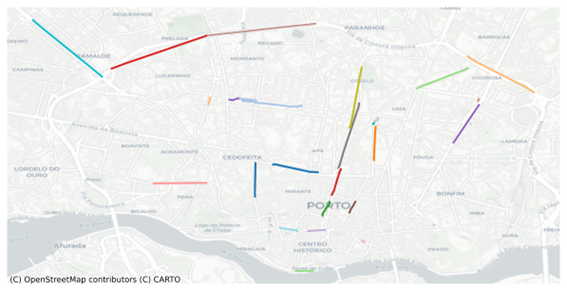
\includegraphics[width=0.5\textwidth]{img/r_tray_DBSCAN.png}
    \caption{Representación de trayectorias.}
    \label{fig:trayectorias_DBSCAN}
\end{figure}

\FloatBarrier

\item \textbf{HDBSCAN}:  
Este algoritmo no requirió ajustes en sus parámetros predeterminados de \texttt{scikit-learn}. Los resultados fueron similares a los de OPTICS en términos de segmentos (2161), aunque el número de clusters fue menor (96) y el porcentaje de segmentos descartados también disminuyó, alcanzando un 53.54\% (1157 segmentos).

\begin{figure}[h!]
    \centering
    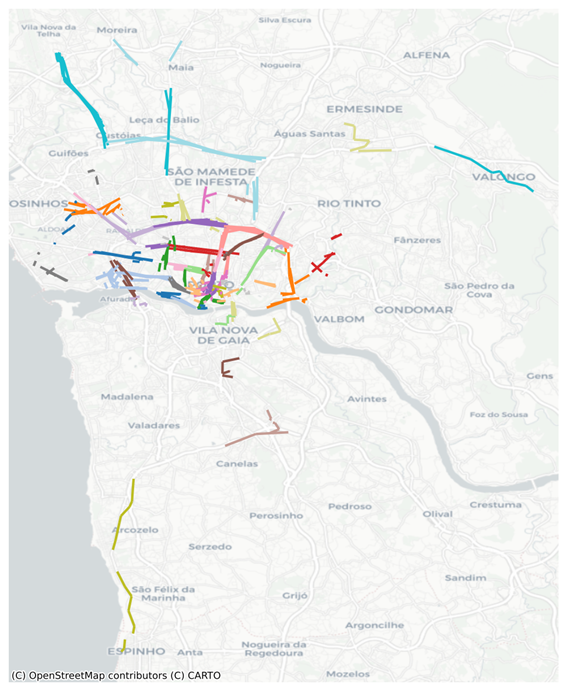
\includegraphics[width=0.5\textwidth]{img/clusters_HDBSCAN.png}
    \caption{Representación de clusters.}
    \label{fig:clusters_HDBSCAN}
\end{figure}

\begin{figure}[h!]
    \centering
    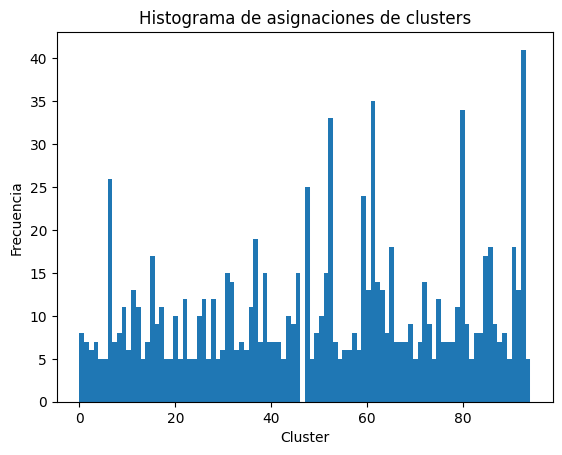
\includegraphics[width=0.5\textwidth]{img/histograma_HDBSCAN.png}
    \caption{Segmentos por cada cluster.}
    \label{fig:histograma_HDBSCAN}
\end{figure}

\begin{figure}[h!]
    \centering
    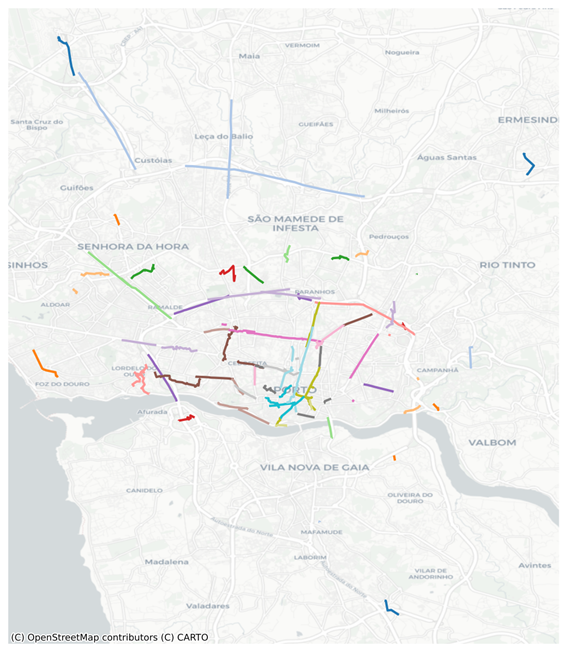
\includegraphics[width=0.5\textwidth]{img/r_tray_HDBSCAN.png}
    \caption{Representación de trayectorias.}
    \label{fig:trayectorias_HDBSCAN}
\end{figure}

\FloatBarrier

\item \textbf{Agglomerative Clustering}:  
Este algoritmo requería definir previamente el número de clusters. En este caso, se utilizaron los 2654 segmentos generados, sin descartar ninguno, ya que no clasifica datos como "basura". Sin embargo, esta característica provoca que los clusters no se centren en las zonas más densas, lo que resulta en representaciones de trayectorias más erráticas.

\begin{figure}[h!]
    \centering
    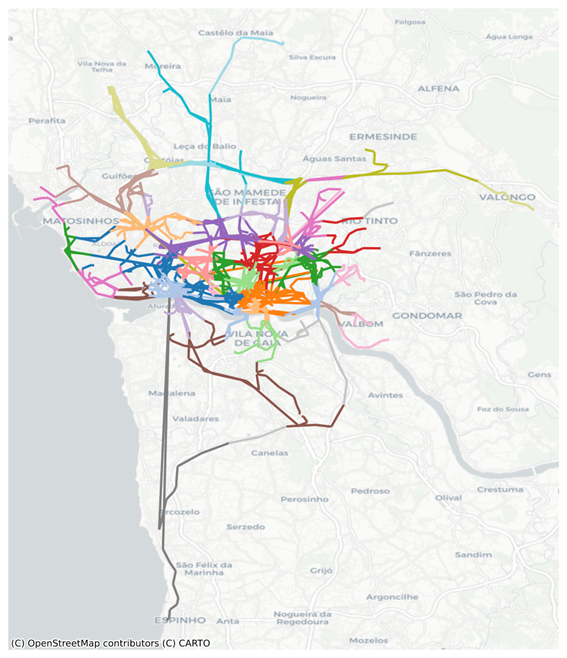
\includegraphics[width=0.5\textwidth]{img/clusters_Aggl.png}
    \caption{Representación de clusters.}
    \label{fig:clusters_Agglomerative}
\end{figure}

\begin{figure}[h!]
    \centering
    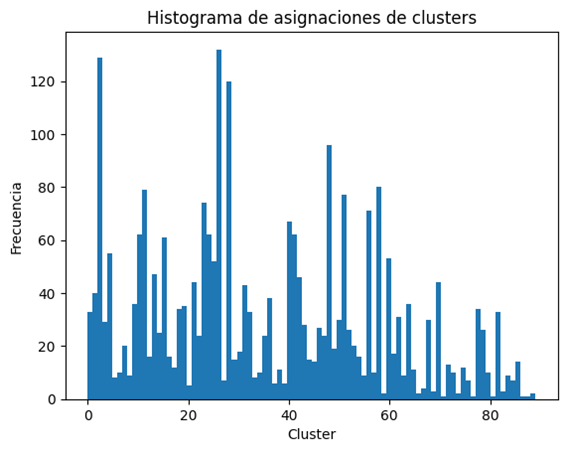
\includegraphics[width=0.5\textwidth]{img/histograma_Aggl.png}
    \caption{Segmentos por cada cluster.}
    \label{fig:histograma_Agglomerative}
\end{figure}

\begin{figure}[h!]
    \centering
    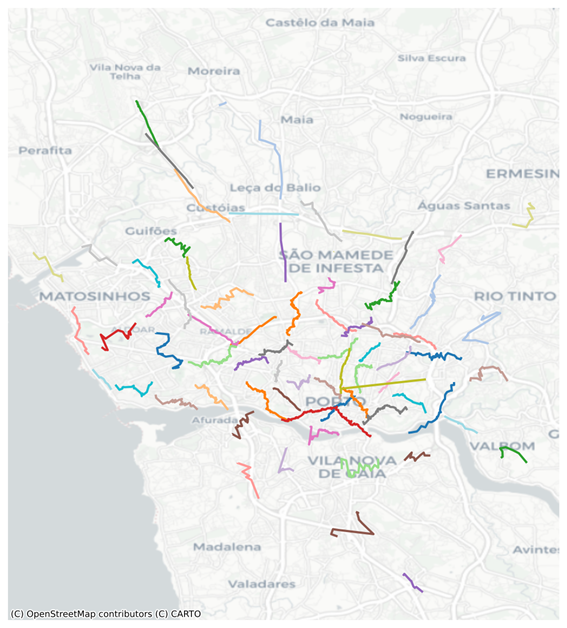
\includegraphics[width=0.5\textwidth]{img/r_tray_Aggl.png}
    \caption{Representación de trayectorias.}
    \label{fig:trayectorias_Agglomerative}
\end{figure}

\FloatBarrier

\item \textbf{Spectral Clustering}:  
Al igual que el algoritmo anterior, no descarta datos. Aunque se generaron los mismos 2654 segmentos y clusters que en Agglomerative Clustering, los resultados finales fueron diferentes, con una distribución menos centralizada.

\begin{figure}[h!]
    \centering
    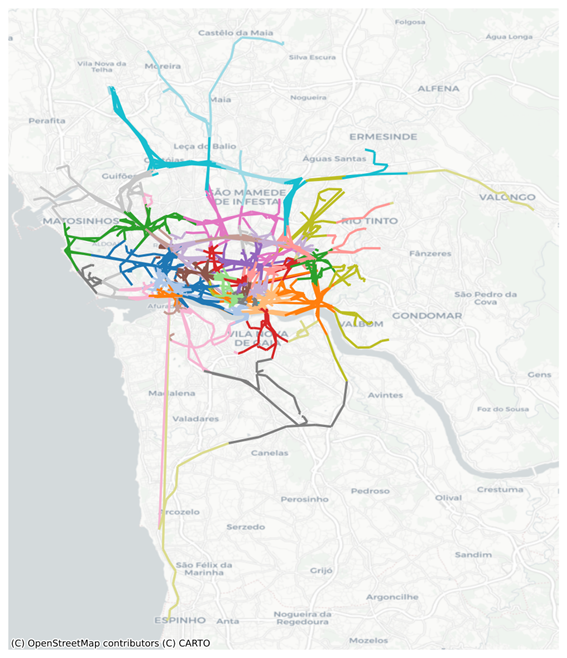
\includegraphics[width=0.5\textwidth]{img/clusters_Spect.png}
    \caption{Representación de clusters.}
    \label{fig:clusters_Spectral}
\end{figure}

\begin{figure}[h!]
    \centering
    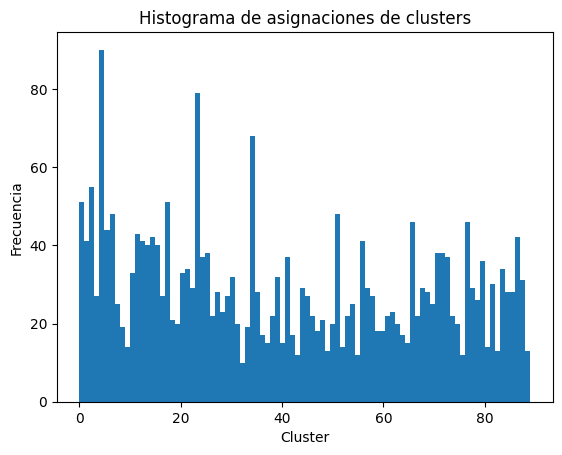
\includegraphics[width=0.5\textwidth]{img/histograma_Spect.png}
    \caption{Segmentos por cada cluster.}
    \label{fig:histograma_Spectral}
\end{figure}

\begin{figure}[h!]
    \centering
    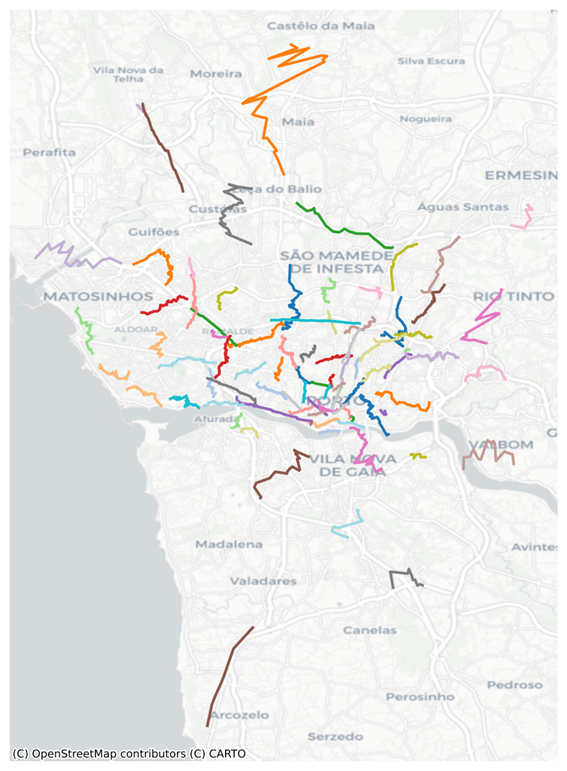
\includegraphics[width=0.5\textwidth]{img/r_tray_Spect.png}
    \caption{Representación de trayectorias.}
    \label{fig:trayectorias_Spectral}
\end{figure}

\FloatBarrier

\end{enumerate}

\subsection{Conclusión}



\section{Pruebas funcionales}

Para demostrar la utilidad del algoritmo y la aplicación creados, se propuso realizar múltiples pruebas con diferentes conjuntos de datos, tamaños y configuraciones aplicados a los algoritmos de clustering.

\subsection{Conjuntos de datos}

Durante el desarrollo del proyecto, se utilizó en prácticamente todo el conjunto de datos de Trayectorias Taxis \cite{trayectorias_taxis}. Para esta comprobación final, esto no era suficiente. Usar solo este conjunto de datos limitaría el proyecto a un análisis específico. Por lo tanto, se buscó encontrar múltiples conjuntos de datos.

Aunque existen multitud de conjuntos de datos con coordenadas GPS que pueden servir la mayoría de ellos no se encuentran en un formato preparado para correr el TRACLUS. Normalmente los conjuntos suelen separar las coordenadas en puntos lo cual no es valido ya que el TRACLUS, este necesita de trayectorias por tanto hay que juntar los datos de forma lógica con un formato valido. 

El primer conjunto con esa estructura adaptada fue Geolife \cite{geolife_trajectories}. Este estudio organiza los datos en carpetas, una por cada sujeto al que se le registraron ubicaciones durante un periodo de tiempo. Dentro de cada carpeta se encontraban varios archivos \texttt{.plt} que contenían información sobre la latitud, longitud, hora y fecha de las mediciones. 

Para organizar los datos de forma lógica para el algoritmo TRACLUS, no era viable crear una fila por cada archivo \texttt{.plt}, ya que algunos contenían más de 1000 mediciones. Por lo tanto, se decidió agrupar las mediciones por hora. Todas las mediciones tomadas dentro de la misma hora se combinaron en una única fila de un archivo Excel.

Se creó una función para automatizar este proceso por carpeta, lo que permitió realizar pruebas fácilmente en diferentes sujetos. Para analizar los resultados, se utilizó un archivo Excel generado con todos los datos encontrados en la carpeta del sujeto \texttt{000}.

Otro conjunto de datos probado fue uno de MoveBank \cite{movebank}, una plataforma que contiene miles de trayectorias de animales. Debido a la inmensidad de opciones disponibles, se seleccionó de forma semi-aleatoria el conjunto de datos titulado \textit{"Hammer-headed fruit bats (Hypsignathus monstrosus) in the Republic of Congo"}. Este conjunto incluía datos de múltiples murciélagos de la fruta registrados en diferentes días. 

Tras analizar el número de mediciones por hora, se decidió dividir las trayectorias por murciélago y día, creando un conjunto de datos con filas más reducidas en comparación al anterior. Aun así, estas filas eran considerablemente más grandes que las del conjunto de Trayectorias Taxis, lo cual incrementó significativamente el tiempo de procesamiento por cada fila analizada.

Ademas de estos tres se hicieron pruebas con otros como Citi Bikes \cite{} o Foursquare-NY \cite{} pero los resultado no fueron visualmente atractivos para un buen analisis y muestra.

\subsection{Criterios para las pruebas:}

\begin{enumerate}
    \item \textbf{Límite de tiempo:} Cada prueba debe durar un máximo de dos horas, considerando tanto el tiempo de ejecución como el de representación de los datos. Este límite puede variar según el tamaño del conjunto de datos y el número de coordenadas procesadas.
    \item \textbf{Selección de parámetros:} No se probarán todas las combinaciones posibles. Se seleccionarán aquellas configuraciones que se consideren más relevantes y que puedan producir cambios significativos en los resultados.
    \item \textbf{Parámetros predeterminados:} En las pruebas que uno de los elementos se cambie el resto de ellos permanecerán con los siguientes valores: 
    
    \begin{itemize}
    		\item \textbf{Metric:} \texttt{euclidean}
    		\item \textbf{Algorithm:} \texttt{auto}
    		\item \textbf{Min\_samples:} 5
   		\item \textbf{Max\_eps:} 1
    		\item \textbf{Eps:} 0.1
    		\item \textbf{Linkage:} \texttt{ward}
    		\item \textbf{Affinity:} \texttt{nearest\_neighbors}
    		\item \textbf{Assign\_labels:} \texttt{kmeans}
    		\item \textbf{n\_clusters:} 7
	\end{itemize}

\end{enumerate}

\subsection{Resultados}

\subsubsection{OPTICS, DBSCAN y HDBSCAN}

En las pruebas iniciales, se observó que, debido a las características de los datos seleccionados, los algoritmos OPTICS y HDBSCAN tendían a comportarse de manera similar, con la principal diferencia siendo el parámetro \texttt{Max\_eps}, esta se calcula internamente en HDBSCAN por lo que dependiendo de la cantidad de datos esta cambiara. Por otro lado, DBSCAN también podría reproducir resultados similares bajo configuraciones específicas del parámetro \texttt{eps}. 

Para comprender cómo los parámetros afectan el rendimiento de cada algoritmo, se realizaron pruebas aislando cada parámetro. Es decir, al modificar un parámetro, los demás permanecieron en sus valores predeterminados.

\paragraph{Métricas (\texttt{metric})}

Las métricas utilizadas para calcular las distancias entre puntos demostraron tener un impacto significativo en los resultados. Los hallazgos principales fueron los siguientes:

- \textbf{Métricas no funcionales}: Algunas métricas, como \texttt{l1} y \texttt{cosine}, no pudieron procesar correctamente los datos seleccionados, lo que resultó en errores o en agrupaciones inadecuadas.
- \textbf{Manhattan}: Esta métrica tendió a considerar todos los puntos como parte de un único clúster grande, resultando en una agrupación poco informativa. En el caso de las trayectorias, esto significó un único grupo, lo que limitó el análisis.












